\documentclass[UTF8, fontset=macnew, a4paper, 12pt]{ctexart}

\usepackage{geometry}
\geometry{top=2.2cm, bottom=2.2cm, left=2.2cm, right=2.2cm}
\usepackage{amsmath, amssymb}
\usepackage{booktabs}
\usepackage{multirow}
\usepackage{tabularx}
\usepackage{graphicx}
\usepackage{caption}
\usepackage{xcolor}
\usepackage{float}
\usepackage{enumitem}
\usepackage{fancyhdr}
\usepackage{setspace}
\usepackage{pifont}
\usepackage{natbib}
% 拉丁作者名之後採半形括號（中文作者名在書目的中文部分仍用全形）；
% 第五個引數留空表示作者與年份之間不加逗號。
\bibpunct{(}{)}{; }{a}{}{,}
\usepackage[hidelinks]{hyperref}

\graphicspath{{../output/figures/}}
\captionsetup{font=small, labelfont=bf, labelsep=quad}
\setlist{itemsep=2pt, parsep=0pt, topsep=4pt}
\singlespacing

% ctexart 預設的圖表標號前綴為簡體「图」，改回正體。
\renewcommand{\figurename}{圖}
\renewcommand{\tablename}{表}

\ctexset{
  section/format = \raggedright\zihao{4}\bfseries,
  section/name   = {},
  section/number = \bignum{\value{section}},
  section/aftername = 、,
  subsection/format = \raggedright\zihao{5}\bfseries,
  subsection/number = \chinese{subsection},
  subsection/aftername = 、,
  subsubsection/format = \raggedright\normalsize\bfseries,
}
\newcommand{\bignum}[1]{\ifcase#1\or 壹\or 貳\or 參\or 肆\or 伍\or
  陸\or 柒\or 捌\or 玖\or 拾\fi}
\renewcommand{\thesection}{\bignum{\value{section}}}
% 交叉引用子節時補上節次，否則 \ref 只印出「三」而無從判斷屬於哪一節。
\renewcommand{\thesubsection}{\chinese{subsection}}
\makeatletter
\renewcommand{\p@subsection}{\thesection 節之}
\makeatother
\setcounter{secnumdepth}{2}

\pagestyle{fancy}
\fancyhf{}
\fancyhead[L]{}
\fancyhead[R]{\small 進度報告（1012 摘要版）}
\fancyfoot[C]{\small \thepage}
\renewcommand{\headrulewidth}{0.4pt}

% U+2460~2463 不在 xeCJK 認定的 CJK 範圍內，會落到拉丁字型而缺字，
% 因此改用 pifont 的圈號。
\newcommand{\cn}[1]{\ding{\number\numexpr171+#1\relax}}
\newcommand{\edag}{e_0^{\dagger}}
\newtheorem{prop}{Proposition}
\newtheorem{cor}{Corollary}
\newtheorem{lem}{Lemma}
\newenvironment{proof}{\par\noindent\textit{Proof}.\ }{\hfill$\square$\par\vspace{4pt}}
\newcommand{\Ex}{\mathbb{E}}

% 分部標題
\newcommand{\partline}[2]{%
  \par\vspace{10pt}\noindent\rule{\textwidth}{0.8pt}\par\vspace{2pt}
  \noindent{\zihao{4}\bfseries 第#1部\quad #2}\par
  \vspace{2pt}\noindent\rule{\textwidth}{0.8pt}\par\vspace{6pt}%
  \phantomsection\addcontentsline{toc}{part}{第#1部\quad #2}}

% 目錄：只收到小節，部次以粗體與一行間距與節次區隔。
\setcounter{tocdepth}{2}
\makeatletter
\renewcommand{\l@part}[2]{\par\vspace{8pt}%
  \noindent{\bfseries #1}\par\vspace{2pt}}
\renewcommand{\l@section}[2]{\@dottedtocline{1}{0em}{5.2em}{\bfseries #1}{\bfseries #2}}
\renewcommand{\l@subsection}[2]{\@dottedtocline{2}{5.2em}{4.6em}{#1}{#2}}
\makeatother

\begin{document}
\pagenumbering{arabic}

\begin{center}
{\zihao{3}\bfseries 小人口 Lee-Carter 參數偏誤的閉式}\\[4pt]
{\zihao{5} ——問題、解決方案與策略（摘要版）}\\[8pt]
{\zihao{5} （林子立）\quad 指導教授：余清祥\,教授\quad 國立政治大學統計學系}\\[4pt]
{\zihao{5} 中華民國 115 年 10 月 12 日}
\end{center}

\vspace{4pt}
\noindent\rule{\textwidth}{0.8pt}
\vspace{2pt}

\noindent 本文為 \texttt{進度報告\_1012\_V1}（74 頁）的摘要，
只保留問題的界定、所提方法與其成績，以及後續的取捨。
各節末標示完整版的對應節次。除第\ref{ss:cross}節的跨國部分
（六國、1998--2021 年）之外，所有數值皆為臺灣女性 2001--2024 年資料、
重複一百次、固定亂數種子。

\vspace{2pt}
\noindent\rule{\textwidth}{0.8pt}

\section{問題}\label{s:prob}

\subsection{現象與既有的處理}

Lee-Carter 模型以 $\log m_{x,t}=\alpha_x+\beta_x\kappa_t$ 刻畫死亡率，
其標準估計是對 $\log\hat m_{x,t}=\log\big(\max(D_{x,t},c_0)/E_{x,t}\big)$
作奇異值分解，其中 $c_0$ 為零死亡時的替代值，慣例取 $0.5$。
人口規模小時該估計的年齡參數有方向明確的偏誤，
既有研究以模擬量化此一現象，並以修勻或參考母體加以緩解。

\textbf{本文的出發點是：該偏誤不是模擬所觀察到的經驗現象，
而是估計方程的一項可以寫出來的性質。}

\subsection{偏誤的閉式與其兩個來源}

$\hat\alpha_x$ 是 $\log\hat m_{x,t}$ 的列平均，而該平均在奇異值分解之前
即已定出。故其偏誤為逐格偏誤的平均，而逐格偏誤有閉式：
$D\sim\text{Poisson}(\mu)$ 時
\begin{equation}\label{eq:b}
b(\mu;c_0)=\Ex[\log\max(D,c_0)]-\log\mu
= e^{-\mu}\log c_0+\sum_{d\ge1}\frac{e^{-\mu}\mu^{d}}{d!}\log d-\log\mu .
\end{equation}
式~\eqref{eq:b} 可再分解為兩項，\textbf{而兩項的成因不同}：
$$b(\mu;c_0)=\underbrace{\pi\log\frac{c_0}{\mu_+}-\log(1-\pi)}_{\text{零格替代}}
-\underbrace{(1-\pi)\big(\log\mu_+-\Ex[\log D\mid D\ge1]\big)}_{\text{Jensen}},$$
其中 $\pi=\Pr(D=0)$、$\mu_+=\Ex[D\mid D\ge1]$。
零格主導 $\mu$ 小的年齡，Jensen 主導 $\mu$ 大的年齡，
而兩者的符號相反，故 $b$ 有唯一的變號點。

\subsection{三個須先認清的性質}

\textbf{其一，這是有限樣本的恆等式，不是漸近近似。} 式~\eqref{eq:b} 不含
觀測年數 $T$，故\textbf{增加觀測年數不使該偏誤消失}；它只隨每格的期望死亡數
$\mu_{x,t}$ 增大而消失。這與 \citet{coxsnell1968} 與 \citet{firth1993}
所處理的 $O(n^{-1})$ 漸近偏誤性質不同。

\textbf{其二，哪些年齡被高估是分析者選出來的。} 變號點 $\mu^{\ast}$ 隨 $c_0$ 移動：
$c_0=0.1/0.3/0.5/1.0$ 分別給出 $\mu^{\ast}=0.134/0.533/0.923/1.509$。
慣例的 $0.5$ 給出 $\mu^{\ast}=0.9234$，即「每年約一人死亡」這個分界。

\textbf{其三，偏誤的位置與量都可在配適之前算出}，
因為式~\eqref{eq:b} 只需要曝露數與一組粗略的死亡率。這一點是第\ref{s:sol}節
事前檢定的基礎。

\subsection{問題的規模}

人數一萬、女性的年齡結構下，期望有 $39.2\%$ 的格為零死亡，
且平均有 $0.90$ 個年齡整列全零；人數五千與兩千時零格佔 $48.7\%$ 與 $63.0\%$。
而我國 368 個鄉鎮市區中有 299 個單一性別人數少於五萬、217 個少於兩萬。

\begin{table}[H]
\centering
\caption{標準 Lee-Carter 的偏誤隨人口規模（重複 100 次的中位數）}
\small
\begin{tabular}{rrrrr}
\toprule
人數 & $\alpha$ 中位偏誤 & $\alpha$ 最大偏誤 & $e_0$ 偏誤（歲） & 整列全零的年齡數\\
\midrule
2{,}000 & 0.8807 & 3.9114 & $-16.92$ & 4.02\\
5{,}000 & 0.2585 & 2.9951 & $-6.88$ & 2.06\\
10{,}000 & 0.1712 & 2.3309 & $-3.73$ & 0.90\\
50{,}000 & 0.0693 & 0.8658 & $-1.47$ & 0.00\\
200{,}000 & 0.0231 & 0.1846 & $-1.22$ & 0.00\\
\bottomrule
\end{tabular}
\label{t:prob}
\end{table}

\begin{figure}[H]
\centering
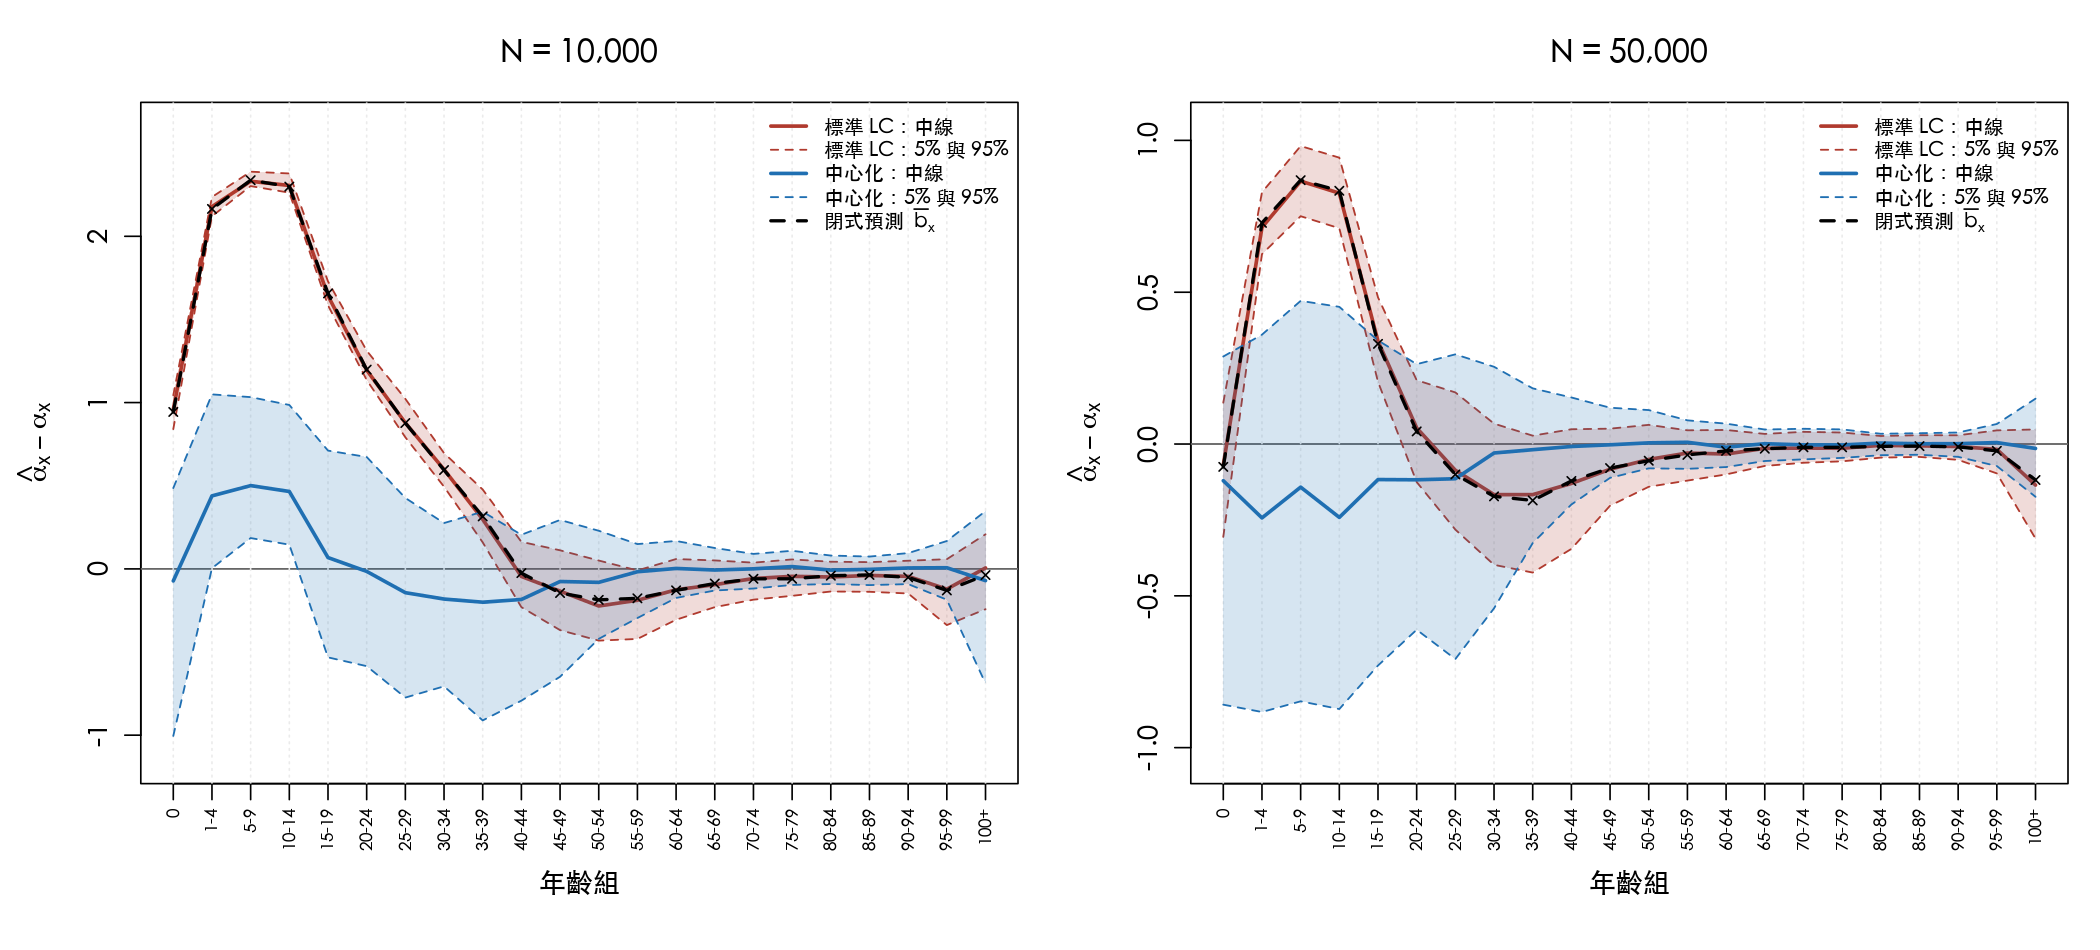
\includegraphics[width=0.82\textwidth]{figT1_alpha_band.png}
\caption{逐年齡的 $\alpha$ 偏誤與其閉式預測（人數五萬）}
\end{figure}

圖中的實線為式~\eqref{eq:b} 所預測的偏誤、點為模擬實測的中位數。
兩者在幼年組同為大的正值、在高齡組同為小的負值，而交叉處即 $\mu^{\ast}$。
\textbf{值得注意的是帶寬與準度的脫鉤}：幼年組的帶最窄而偏離最遠。

\noindent（完整版第壹、貳、參節）

\subsection{資料與驗證的設計}\label{ss:data}

全部分析使用內政部與衛福部的臺灣死亡與人口資料，女性 2001--2024 年、
二十二個年齡組（$0$、$1$--$4$、$5$--$9$、\ldots、$100^{+}$），共 $22\times24$ 格。
只用女性，因其死亡率曲線較平滑，可使閉式的驗證不混入模型誤設。
依既定方針不作單齡組的分析。

驗證以兩種方式進行。其一是\textbf{模擬}：以全國資料的 Poisson 配適為真值，
按該年齡結構縮放至指定人數後模擬 Poisson 死亡數。
此法的代價是它假設小人口的死亡率恰好等於全國的死亡率，
而真實的鄉鎮市區顯然不是如此；但本文此處的目的是檢驗閉式，
而閉式所刻畫的是估計程序對給定 $\mu_{x,t}$ 的反應。
其二是\textbf{二項抽薄}：由實際的全國死亡數抽薄至小人口，
如此保留臺灣死亡率的逐年不規則性，用於模型誤設下的穩健性檢驗。

一律重複一百次、固定亂數種子，並\textbf{以中位數而非平均數匯總}，
使少數發散的重複不致主導結論。
邊界配適如實保留而不剔除、不重抽；其出現頻率系統性回報如下
（\citealp{pawel2026} 指出 482 篇模擬研究中只有 $23\%$ 提到演算法失敗）。

\begin{table}[H]
\centering
\caption{整列零死亡與邊界配適的出現頻率（Poisson 最大概似，100 次重複）}
\small
\begin{tabular}{rrr}
\toprule
人數 & 整列全零的年齡數 & 出現邊界配適的重複次數\\
\midrule
2{,}000 & 4.02 & 87\\
5{,}000 & 2.06 & 98\\
10{,}000 & 0.90 & 93\\
50{,}000 & 0.00 & 5\\
200{,}000 & 0.00 & 0\\
\bottomrule
\end{tabular}
\label{t:bnd}
\end{table}

\textbf{人數一萬時一百次重複中有 93 次至少一個年齡落在邊界}，
故這不是偶發的極端值而是該規模下的常態。
人數五萬時已無整列全零卻仍有 5 次發散，
可知接近全零而非恰好全零亦足以使解發散。

\section{解決方案}\label{s:sol}

\subsection{閉式的驗證}

以 $\mathrm{mean}_t\,b(\mu_{x,t})$ 預測標準 Lee-Carter 的逐年齡 $\alpha$ 偏誤，
對照模擬實測，逐年齡相關係數在人數 $10^4$、$5\times10^4$、$2\times10^5$ 時
為 $1.000$、$1.000$、$0.988$，迴歸斜率為 $1.001$、$0.990$、$0.962$，
殘差落在蒙地卡羅誤差的量級。
\textbf{亦即標準 Lee-Carter 的 $\alpha$ 偏誤可由單一個死亡數的函數完全解釋。}

\subsection{二階解析量與效率的上界}

除偏誤之外另導出三個量，全部為截斷精確和、已通過數值核對：
對數尺度的變異數 $v(\mu;c_0)=\mathrm{Var}[\log\max(D,c_0)]$、
偏誤的導數 $b'(\mu;c_0)$，以及估計方程的靈敏度 $A(\mu)=1+\mu b'(\mu)$。
由此得到一個可寫成恆等式的結果：相對於 Poisson 最大概似的效率為
$\mathrm{corr}\big(\log\max(D,c_0),\,D\big)^2$，其值全程不低於 $0.8776$。
\textbf{亦即取對數與零格替代合起來的效率損失不超過 $12.2\%$}——
問題在偏誤，不在效率。

另一項對實務有用的性質：$v(\mu;c_0)$ 對 $\mu$ 非單調，於 $\mu\approx2$ 取極大
（$v(0.02)=0.0096$、$v(2)=0.480$、$v(300)=0.0034$）。
零格主導的年齡其估計帶很窄卻離真值很遠，\textbf{「帶窄」與「準」在此完全脫鉤}。

\subsection{卜瓦松假設是否要緊}

式~\eqref{eq:b} 依賴卜瓦松假設，而真實死亡數可能過度離散。
本文把偏誤寫成一般形式之後，此一問題可以直接回答：
零格替代那一項只依賴 $\pi=\Pr(D=0)$ 與 $\mu_+$，
而 Jensen 那一項在過度離散下由 $1/(2\mu)$ 變為 $\phi/(2\mu)$。
以負二項取代卜瓦松重算變號點：
$$\phi=1.0\Rightarrow\mu^{\ast}=0.9234,\qquad
\phi=1.5\Rightarrow0.8690,\qquad
\phi=2.0\Rightarrow0.8289 .$$
\textbf{變號點只移動不到一成，故本文的診斷對卜瓦松假設並不敏感。}
此一結果使閉式可用於真實資料，而不必先檢定離散程度。

\subsection{事前可行性檢定與分級}

既然偏誤只需曝露數與粗略死亡率即可算出，本文把它包裝成一個
\textbf{不需模擬、不需真值、也不需參考母體}的事前檢定，並分四級。
以臺灣女性 2001--2024 年的年齡結構與死亡率計算，
單一性別人數兩萬四千以下為 D 級、九萬六千以上為 B 級。
\textbf{該兩個數字須連同其所依據的年窗與年齡結構一併引用，不是普遍的門檻}：
改用 1998--2021 的年窗重算，B 級門檻由 $95{,}773$ 降為 $77{,}902$，
相差 $23\%$，因為期間死亡率下降而使各格更空。

門檻本身有一行精確的解。由 $\mu_{x,t}=N\,w_x\,m_{x,t}$（$w_x$ 為年齡結構），
分級所用的佔比 $\mathrm{mean}(\mu_{x,t}<\mu^{\ast})$ 只透過
$\{w_x m_{x,t}\}$ 的分布進入，解 $N$ 即得
\begin{equation}\label{eq:thresh}
N_p=\frac{\mu^{\ast}}{q_p},\qquad
q_p=\{w_x m_{x,t}\}\ \text{的}\ p\ \text{分位數},
\end{equation}
其中 $p$ 為該級的佔比門檻。$q_p$ 可讀為「每人每格的期望死亡數」，
而 $N_p$ 即\textbf{使第 $p$ 分位的那一格恰好達到 $\mu^{\ast}$ 的人口規模}。
\textbf{式~\eqref{eq:thresh} 使分級可以搬到任何地區}，
所需的輸入只有該地區的年齡結構與一組粗略的死亡率。

此一檢定補上了古典信賴度標準所缺的一半。全信賴度把資料量換算為期望索賠次數
（$k=5\%$、$p=90\%$ 時約 $1{,}082$ 件），\textbf{但它控制的是估計的變異，
而其推導假設估計量無偏}；該假設在此不成立，而本文的門檻正是偏誤側的對應物。

\begin{figure}[H]
\centering
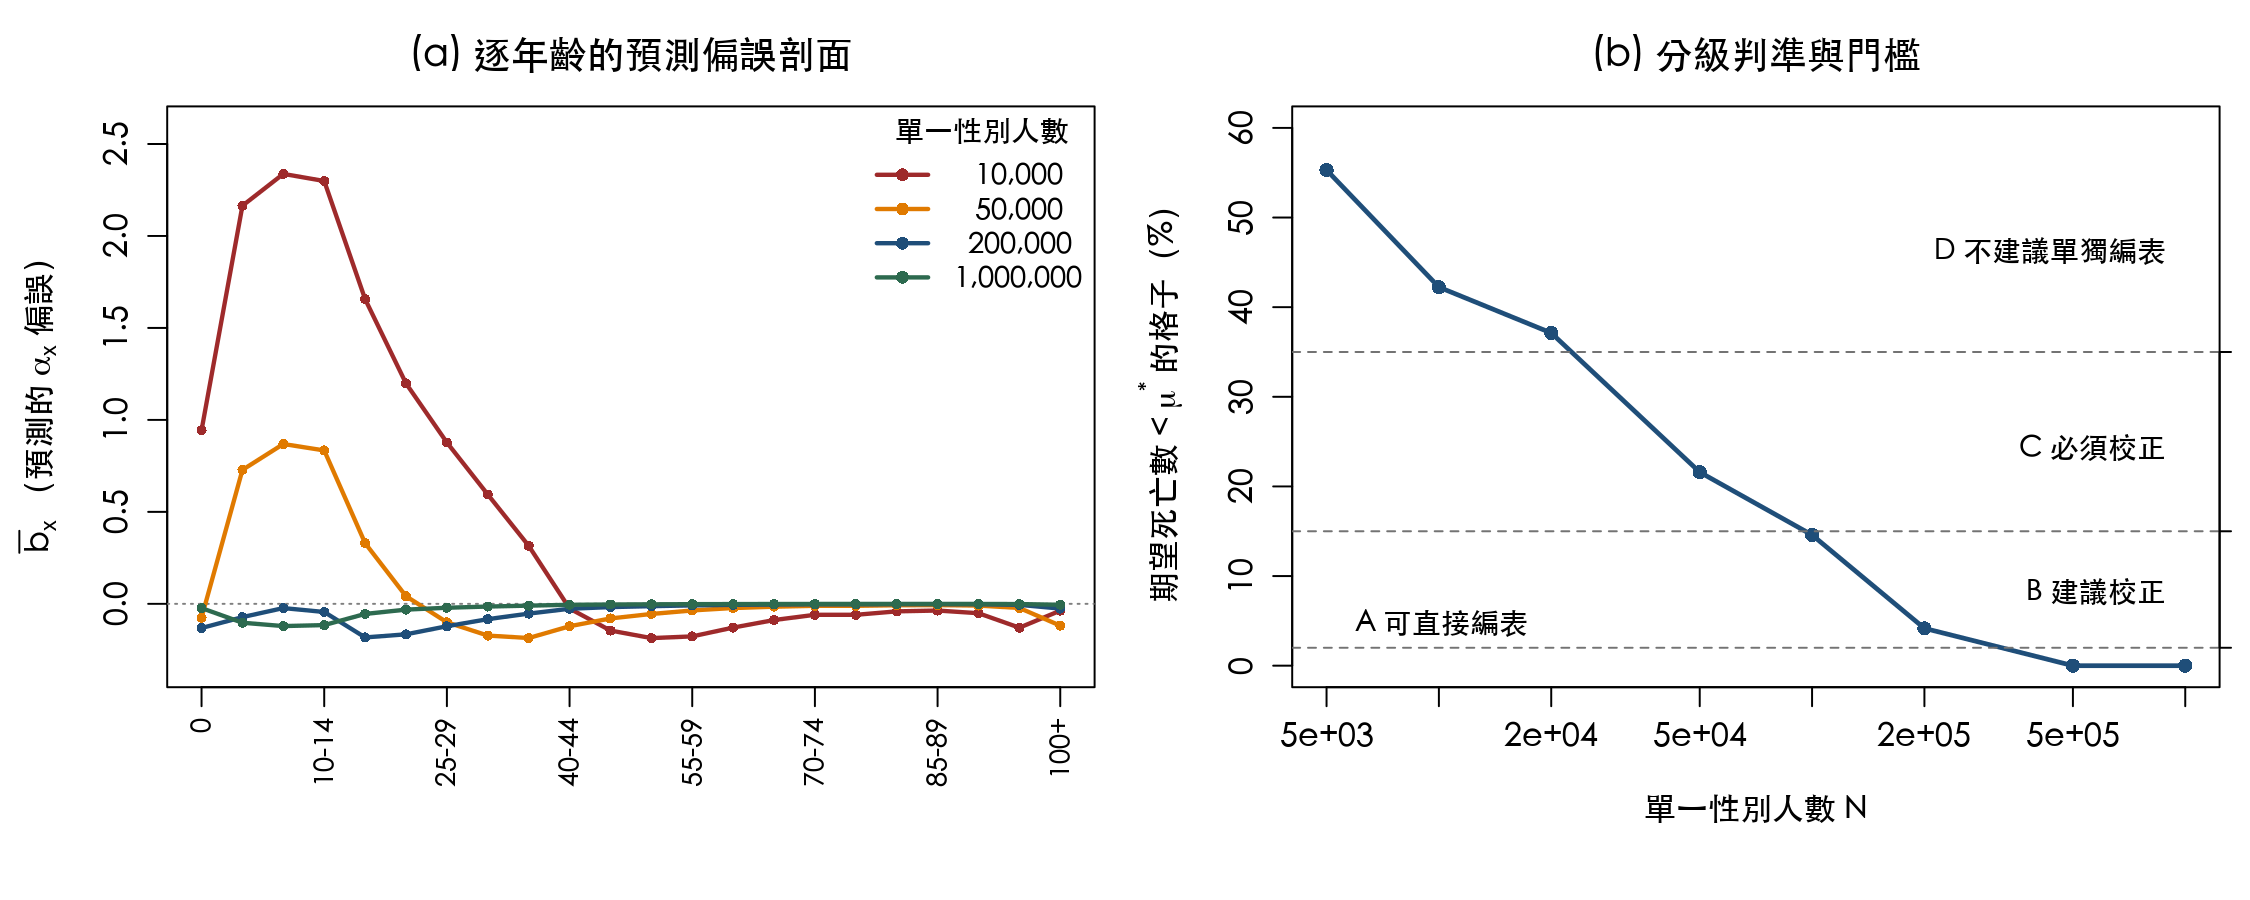
\includegraphics[width=0.80\textwidth]{figF1_feasibility.png}
\caption{事前可行性檢定的四級分級與臺灣鄉鎮市區的分布}
\end{figure}

該分級只用兩個輸入：各年齡的曝露數與一組粗略的死亡率。
其判讀方式與信賴度標準相同——把資料量換算為一個門檻——
但所控制的是偏誤而非變異。

\subsection{校正：只校正 $\alpha$，以資訊加權處理 $\beta$ 與 $\kappa$}

偏誤可預測即可扣除。本文的設計有兩個要點。其一，\textbf{只把 $\bar b_x$ 扣在
$\hat\alpha_x$ 上而完全不動中心化矩陣}，如此 $\hat\beta$ 與 $\hat\kappa$
不受 $\hat\mu$ 的噪音注入。其二，以期望死亡數加權求解秩一結構。

\textbf{兩項改善可以疊加，而其成因已查明。} 以 $2\times2$ 的設計分開施作：
只中心化時 $\beta$ 與 $\kappa$ 的四項指標到小數第四位不動；
只加權時 $\alpha$ 的最大偏誤亦幾乎不動（$0.8658\to0.8660$）。
\textbf{兩者的作用域互不重疊，而分離是精確的}，
因為加權修正的是變異函數（一階），中心化修正的是轉換的偏誤（二階）。

\begin{table}[H]
\centering
\caption{人數五萬時各法的比較（重複 100 次的中位數）}
\small
\begin{tabular}{lrrrrr}
\toprule
估計量 & $\alpha$ 中位 & $\alpha$ 最大 & $\mathrm{SSE}(\beta)$ & 漂移偏誤 & $e_0$ 偏誤\\
\midrule
標準 Lee-Carter & 0.0693 & 0.8658 & 5.9523 & $+0.3327$ & $-1.472$\\
Poisson 最大概似 & 0.0080 & 0.1945 & 1.4098 & $-0.0043$ & $-0.186$\\
Firth 預先修正 & 0.0060 & 0.0733 & 1.2156 & $\mathbf{+0.0023}$ & $-0.251$\\
本文（中心化＋加權） & 0.0193 & 0.0768 & \textbf{1.1586} & $+0.1362$ & $\mathbf{-0.041}$\\
本文（分離式） & \textbf{0.0067} & \textbf{0.0391} & 1.1762 & $+0.1357$ & $+0.273$\\
\bottomrule
\end{tabular}

\vspace{2pt}
\parbox{0.92\textwidth}{\footnotesize 註：分離式指 $\hat\alpha_x$ 維持等權列平均、
加權只用於秩一結構，為本輪新增的設計。}
\label{t:main}
\end{table}

\subsection{平均餘命與時間參數}

$e_0$ 是實務上真正要看的量，而本文的修正在該量上有一項值得指出的性質：
人數五萬時 $e_0$ 偏誤由 $-1.48$ 歲降到 $-0.04$ 歲，
而其標準差由 $0.585$ 只變為 $0.644$。\textbf{偏誤的移除沒有付出相稱的變異代價。}
但 Firth 的均方根誤差仍較小（$0.513$ 對 $0.644$），
故在 $e_0$ 上兩法各有勝負。

時間參數則有一項須明寫的限制。$\hat\kappa_t$ 的全距被壓縮，
而該壓縮須拆成兩件事才不致誇大：

\begin{table}[H]
\centering
\caption{$\hat\kappa$ 的衰減與形狀（真值全距 $9.850$）}
\small
\begin{tabular}{llrrr}
\toprule
人數 & 估計量 & 逐次全距中位 & 中位路徑全距 & $\mathrm{cor}(\hat\kappa,\kappa)$\\
\midrule
一萬 & 標準 Lee-Carter & 5.183 & 1.576 & 0.340\\
一萬 & 中心化＋加權 & 8.598 & 4.446 & 0.698\\
五萬 & 標準 Lee-Carter & 5.602 & 1.785 & 0.393\\
五萬 & 中心化＋加權 & \textbf{7.620} & 6.555 & \textbf{0.941}\\
\bottomrule
\end{tabular}
\label{t:kappa}
\end{table}

\textbf{逐次的全距衰減到五成三至五成七，而各次 $\hat\kappa$ 的中位路徑
其全距只有一成六至一成八}——後者小得多，是因為標準 Lee-Carter 各次的形狀
彼此不一致（與真值的相關只有 $0.34$ 至 $0.39$），中位數因而互相抵銷。
只引中位路徑的壓縮比例會把衰減說得過重。
而加權把形狀大幅修回（五萬時相關 $0.393\to0.941$），
故「校正後的時間路徑擺幅更大」在該規模上是衰減更少而非缺陷。

\subsection{與參考母體修勻法的對照}

既有的緩解手段是修勻與參考母體，故須與之比較。
以 \citet{lee2003} 的 partial SMR 為代表、人數五萬、參考母體兩百萬：

\begin{table}[H]
\centering
\caption{與參考母體法的比較（$\alpha$ 偏誤中位數）}
\small
\begin{tabular}{lrrr}
\toprule
情境 & Partial SMR & Whittaker 比值修勻 & 本文（中心化＋加權）\\
\midrule
年齡型態相同 & \textbf{0.0025} & 0.0095 & 0.0223\\
型態遞增 & 0.2064 & 0.0100 & \textbf{0.0223}\\
型態遞減 & 0.3313 & 0.0123 & \textbf{0.0223}\\
\bottomrule
\end{tabular}

\vspace{2pt}
\parbox{0.92\textwidth}{\footnotesize 註：本文的方法不使用參考母體，
故三個情境下的結果相同。}
\label{t:smr}
\end{table}

\textbf{參考母體的型態與目標區域相符時 partial SMR 明顯較優，
型態不符時其 $\alpha$ 偏誤惡化至本文的九至十五倍。}
前者應視為該法的上界而非實務可期待的表現，蓋因該情境下
$\mathrm{SMR}\cdot m^{R}_x$ 幾乎就是真值。
\textbf{本文方法的位置因而清楚：它不需要參考母體，
故在找不到型態相符的參考母體時是可用的那一個。}

另附一項分解：只把零格由 $c_0/E$ 改填 $\mathrm{SMR}_t\cdot m^{R}_{x,t}$、
其餘各格完全不動，即可移除約一半的偏誤（$\alpha$ 最大偏誤 $0.866\to0.332$）。
\textbf{剩下的一半來自非零格的 Jensen 項，而那一部分只有中心化能處理}——
這是對第\ref{s:prob}節兩項分解的另一個支持。

\subsection{跨國的適用性}\label{ss:cross}

本文的方法是否也適用於其他地區，答案分三層，而只有第三層是限制。
資料為人類死亡率資料庫的澳洲、加拿大、日本、紐西蘭、美國，加臺灣共六國，
女性 1998--2021 年、同樣的 22 個年齡組。

\textbf{第一層，閉式逐國成立，而且理由是先驗的。}
$b(\mu;c_0)$ 只依賴 $\mu$ 與 $c_0$——它是卜瓦松分布的性質，
不是任何國家的性質，故不需要任何重新推導或重新校準。

\begin{table}[H]
\centering
\caption{閉式的跨國驗證與校正的成績（人數一萬，重複 100 次）}
\small
\begin{tabular}{lrrrrrr}
\toprule
國家 & 零格佔比 & 閉式相關 & 閉式斜率 & 標準 $\alpha$ 最大 & 分離式 & Firth\\
\midrule
日本 & 0.430 & 0.9999 & 1.002 & 2.7959 & 0.9712 & 0.2663\\
加拿大 & 0.409 & 0.9999 & 0.993 & 2.4135 & 0.5889 & 0.2451\\
澳洲 & 0.390 & 0.9999 & 1.000 & 2.3357 & 0.5110 & 0.1626\\
紐西蘭 & 0.381 & 0.9999 & 0.994 & 2.1316 & 0.3070 & 0.1771\\
臺灣 & 0.364 & 0.9999 & 0.997 & 2.2546 & 0.4757 & 0.1951\\
美國 & 0.273 & 0.9998 & 0.993 & 2.0257 & 0.3048 & 0.1120\\
\bottomrule
\end{tabular}

\vspace{2pt}
\parbox{0.92\textwidth}{\footnotesize 註：人數五萬時閉式的相關為
$0.9985$ 至 $0.9999$、斜率 $0.980$ 至 $1.002$。}
\label{t:cross}
\end{table}

\textbf{校正在六國皆有效}（分離式把 $\alpha$ 最大偏誤改善 $4.4$ 至 $7.0$ 倍），
而\textbf{Firth 在六國的 $\alpha$ 最大偏誤上皆勝出}，
故第\ref{s:sol}節該項結論不是臺灣資料的特性。

\textbf{第二層，門檻逐國不同，但重算只需式~\eqref{eq:thresh}。}

\begin{table}[H]
\centering
\caption{各國的分級門檻（單一性別人數）}
\small
\begin{tabular}{lrrrr}
\toprule
國家 & $e_0$ & 粗死亡率 & B 級門檻 & C 級門檻\\
\midrule
日本 & 87.56 & 0.00864 & 132{,}436 & \textbf{45{,}516}\\
澳洲 & 85.47 & 0.00635 & 74{,}371 & 22{,}566\\
臺灣 & 84.01 & 0.00515 & 77{,}901 & 22{,}268\\
加拿大 & 84.18 & 0.00714 & 70{,}420 & 21{,}368\\
紐西蘭 & 84.05 & 0.00666 & 49{,}051 & 20{,}362\\
美國 & 80.42 & 0.00832 & 50{,}816 & \textbf{14{,}462}\\
\bottomrule
\end{tabular}
\label{t:thresh}
\end{table}

\textbf{日本的門檻是美國的 $3.1$ 倍}，亦即同一個方法在日本要兩三倍大的地區
才可用。而\textbf{粗死亡率不是預測因子}——日本的粗死亡率最高而門檻也最高、
臺灣最低而門檻居中；驅動因素是\textbf{幼年與中年的死亡率水準}
（日本該段極低故其格最空、美國該段較高故最滿）。
\textbf{亦即本方法在死亡率愈低的地區愈難用，而那正是先進國家的方向。}

\textbf{第三層，兩個模型假設逐國差異很大，而這才是真正的限制。}
秩一佔比由紐西蘭的 $0.5501$、美國的 $0.6230$、加拿大的 $0.6705$
到臺灣的 $0.8962$；而 $\hat\kappa_t$ 對時間的線性 $R^2$ 在五國為
$0.95$ 至 $0.98$，\textbf{美國卻只有 $0.7114$}，
對應已充分記載的美國死亡率在 2010 年代的停滯與反轉。
\textbf{這兩項分別是「對數死亡率在年齡上近於一次式」（即 Gompertz 法則）
與「在時間上近於一次式」（即固定漂移）這兩個假設}，
而它們也正是修勻的差分懲罰其零空間所要求的兩個條件，
故跨國所遇到的限制與本研究另一條線索（修勻）所導出的條件是同一組。

\subsection{估計流程}\label{ss:algo}

為使本摘要可據以實作，此處列出完整的流程。

\begin{table}[H]
\centering
\small
\begin{tabular}{p{0.93\textwidth}}
\toprule
\textbf{輸入}：死亡數 $D_{x,t}$、曝露數 $E_{x,t}$（$A=22$ 個年齡組、
$T=24$ 年）、零格替代值 $c_0=0.5$。\\
\midrule
\textbf{0.\ 事前檢定（配適之前）}：以曝露數與一組粗略的死亡率算出
$\mu_{x,t}$，取低於 $\mu^{\ast}=0.9234$ 的格數佔比，依 $2\%$／$15\%$／$35\%$
分為 A 至 D 級。門檻亦可由 $N_p=\mu^{\ast}/q_p$ 直接算出。\\
\textbf{1.\ 起始}：$\ell_{x,t}=\log\big(\max(D_{x,t},c_0)/E_{x,t}\big)$，
以標準 Lee-Carter（列平均加奇異值分解）取得
$(\hat{\boldsymbol\alpha},\hat{\boldsymbol\beta},\hat{\boldsymbol\kappa})$。\\
\textbf{2.\ 期望死亡數}：$\hat\mu_{x,t}
=E_{x,t}\exp(\hat\alpha_x+\hat\beta_x\hat\kappa_t)$。\\
\textbf{3.\ 校正 $\alpha$}：$\hat\alpha_x\leftarrow
\overline{\ell_{x,\cdot}}-\overline{b(\hat\mu_{x,\cdot};c_0)}$，
\textbf{其中兩個平均皆為等權}（閉式正是對等權列平均成立）。\\
\textbf{4.\ 加權求解秩一結構}：以 $W_{x,t}=\hat\mu_{x,t}/\bar{\hat\mu}$
為權重，對 $(\ell_{x,t}-\hat\alpha_x)\sqrt{W_{x,t}}$ 作奇異值分解，
取第一對奇異向量，並依 $\sum_x\hat\beta_x=1$、$\sum_t\hat\kappa_t=0$ 正規化
（建議另加 $\hat\beta_x\ge0$，見第\ref{ss:norm}節）。\\
\textbf{5.\ 迭代}：回到步驟 2，直至參數的變動小於 $10^{-9}$（實測 3 至 6 次）。\\
\midrule
\textbf{失敗的處理}：不剔除、不重抽，一律保留，並以中位數而非平均數匯總。
邊界配適的出現頻率須系統性回報（見第\ref{ss:data}節）。\\
\textbf{匯總}：重複 $\ge100$ 次、固定亂數種子；關鍵比較須附蒙地卡羅標準誤。\\
\bottomrule
\end{tabular}
\end{table}

步驟 3 的「等權」一項是本輪新增的設計。前此 $\hat\alpha_x$ 亦以 $W$ 加權，
而第\ref{s:sol}節的 $2\times2$ 顯示加權雖改善 $\beta$ 與 $\kappa$
卻使 $\alpha$ 略差；既然變異函數只關係到秩一結構的求解，
把加權限制於步驟 4 即可兩者兼得。

\subsection{Firth 的具體形式，以及它與零格替代的關係}

對照方法中最強的是 \citet{firth1993}，其在本模型下的形式值得寫出，
蓋因它說明了為何它在 $\alpha$ 上勝出。以 Jeffreys 先驗懲罰對數概似
$\ell^{*}=\ell+\tfrac12\log\det I(\theta)$，其修正後的估計方程為
$$\sum_{x,t}\Big(D_{x,t}+\tfrac12 h_{x,t}-\mu_{x,t}\Big)
\frac{\partial\eta_{x,t}}{\partial\theta_r}=0,$$
其中 $h_{x,t}$ 為帽子矩陣的對角元。
\textbf{亦即 Firth 的修正就是把死亡數換成 $D_{x,t}+\tfrac12 h_{x,t}$。}
由 $\mathrm{tr}(H)=p$ 可知所加總量恆為 $p/2$；單一樣本時 $h=1$、
調整恰為 $+\tfrac12$，此即 \citet{haldane1956} 的加常數。

\textbf{關鍵的對照在零死亡的整列上。} 年齡 $x$ 有兩個專屬參數，
故該列的槓桿和趨於 $2$、所加總量為 $1$，於是 Firth 使一整列零死亡的行為
如同\textbf{該列合計有一個死亡}；而標準 Lee-Carter 的 $c_0=0.5$ 是\textbf{逐格}的，
該列合計 $T\times0.5=12$ 個。\textbf{兩者相差 $T=24$ 倍}，
而 $\log 24=3.18$ 正是兩法在該年齡 $\hat\alpha_x$ 之差的量級。

由此得到一個定位：\textbf{Firth 並非與零格替代不同類的方法，
而是一個隱含替代值由模型定出、而非由分析者選定的零格替代}，
且其每格的替代量比慣例小 $T$ 倍。本文對 $c_0$ 任意性的批評在 Firth 上不適用，
代價是其替代值無法調整，且依 \citet{lewis2024}，
最大概似估計量不存在時 Firth 的行為沒有理論保證。

\noindent（完整版第參至捌節；Firth 的推導為第柒節之二）

\subsection{一個結構性的病灶，與一個不花成本的修法}\label{ss:norm}

Firth 既是本文的主要對照，其在本模型下的\textbf{存在性}須查清楚，
而查下去得到一個與正規化有關的結果。

\textbf{其一，Jeffreys 懲罰概似在本文的維度下無上界。}
沿 $\boldsymbol\beta\to\infty$、$\boldsymbol\kappa\to0$ 而 $\eta$ 仍收斂的路徑，
$$\ell_J(\theta(s))=\ell(\eta_\infty)+(T-A-1)\log s+O(1),$$
故 $T\ge A+2$ 時對\textbf{任何}資料 $\sup\ell_J=+\infty$。
本文的 $A=22$、$T=24$ 恰落在該區間。數值核對：$\log\det I$ 對 $\log s$
的斜率為 $1.941$（理論 $2(T-A-1)=2$），而該路徑上對數概似收斂、
$\tfrac12\log\det I$ 每十倍上升 $2.30$，故合計無上界。
\textbf{亦即 \citet{kosmidis2021} 就二項反應所證的有限性不能移植到
Lee-Carter，而本文所報的 Firth 結果是「由奇異值分解的起點出發所達到的
局部根」}，並非全域的最大值。這一點須與 \citet{lewis2024} 的
「最大概似估計量不存在時 Firth 的行為沒有理論保證」並讀。

\textbf{其二，成因是正規化而非資料，而三個常被混用的約束必須分開。}

\begin{enumerate}[label=(\roman*)]
\item $\sum_x\beta_x=1$，一個\textbf{仿射超平面}；
\item $\sum_x|\beta_x|=1$，即 $L^1$ 的單位球面；
\item $\|\boldsymbol\beta\|_2=1$，即 $L^2$ 的單位球面。
\end{enumerate}

\textbf{只有 (i) 不是範數約束}：它不限制 $\boldsymbol\beta$ 的大小，
蓋因正負可以相消。沿上述路徑 $\sum_x\beta_x=1$ 恆成立，
而 $\sum_x|\beta_x|$ 與 $\|\boldsymbol\beta\|_2$ 皆線性發散
（$s=10^5$ 時為 $10^5$ 與 $2.6\times10^4$）。(ii) 與 (iii) 的可行集為緊緻，
故皆封住該路徑；改以 (iii) 表示同一條路徑時，$\log\det I$ 收斂至 $161.617$。
\citet{hunt2020} 已在一般層次指出識別約束是任意的、且會造成配適時的
穩健性問題，並明言其所用的是 $L^1$ \textbf{範數}；
本文所用的 $\sum_x\beta_x=1$ 則是 (i)。

\textbf{其三，而對本文的資料，修法不花成本。}
全國配適的 $\hat\beta_x$ 落在 $0.0078$ 至 $0.1066$、\textbf{無一為負}，
故 $\sum_x|\beta_x|=\sum_x\beta_x=1.0000$——(i) 與 (ii) 在真值處重合。
於是只要保留 $\sum_x\beta_x=1$ 而加上 $\beta_x\ge0$，
可行集即由仿射超平面變為\textbf{單純形}、因而緊緻，
\textbf{而 $\boldsymbol\beta$ 與 $\boldsymbol\kappa$ 的尺度完全不變、
已報告的所有數值一概不動}。改用 (iii) 雖同樣可行，
但會改動所有 $\hat\beta_x$ 與 $\hat\kappa_t$ 的尺度，代價較大而無額外好處。

\subsection{插入式誤差的方法論歸屬}\label{ss:plugin}

本文扣除的是 $b(\hat\mu)$ 而非 $b(\mu)$，而該誤差有明確的歸屬。
以 $\hat\mu$ 代入一個本該在 $\mu$ 處求值的修正量，
其所生的誤差即小區域估計文獻所稱的\textbf{插入式誤差}；
\citet{lahiri2023} 指出「一個二階無偏估計量的函數並不必然是二階無偏的」，
而 \citet{jiang2026} 把標準作法寫成兩步——先取插入式估計量，
再對其偏誤作第二步的修正。
\textbf{本文的設定與該結構相同，差別在於本文的修正量 $b$ 有閉式而該文獻的
變異成分沒有}，故本文能把展開寫出來：
$$\Ex[b(\hat\mu)]-b(\mu)=b'(\mu)\big(\Ex[\hat\mu]-\mu\big)
+\tfrac12 b''(\mu)\mathrm{Var}(\hat\mu)+\cdots$$
而依 \citet{chernozhukov2018} 的語彙，本文的修正\textbf{不是}
Neyman 正交的——$\partial b/\partial\log\mu=A(\mu)-1\to-1$ 而非趨於零——
故插入式誤差進入一階。\textbf{這是本文須正面處理它，
而不能以「$\hat\mu$ 收斂即可」帶過的理由。}

\section{策略}\label{s:strat}

\subsection{哪一項結果管到哪一個參數}\label{ss:map}

本文最容易被誤讀之處是把 $\alpha_x$ 的恆等式當成「小人口 Lee-Carter 偏誤
的一般解」。下表把各項結果的適用範圍逐一標明。

\begin{table}[H]
\centering
\caption{結果與參數的對應}
\small
\renewcommand{\arraystretch}{1.15}
\begin{tabular}{p{4.6cm}ccc}
\toprule
結果 & $\alpha_x$ & $\beta_x$ & $\kappa_t$／漂移\\
\midrule
偏誤的閉式 $b(\mu;c_0)$ & \textbf{恆等式} & 不適用 & 不適用\\
變異數的閉式 $v(\mu;c_0)$ & \textbf{恆等式} & 不適用 & 不適用\\
效率下界 $0.8776$ & 逐格、非參數層 & 不適用 & 不適用\\
事前可行性檢定 & \textbf{直接} & 間接 & 不適用\\
中心化校正 & \textbf{直接} & 不動 & 不動\\
資訊加權 & 不動 & \textbf{直接} & \textbf{直接}\\
對偏離秩一的穩健性 & \textbf{已驗證} & 未驗證 & 未驗證\\
偏誤的解析刻畫 & 有 & 數值分解（確定性成分佔 $9.2\%$） & \textbf{無}\\
\bottomrule
\end{tabular}
\label{t:map}
\end{table}

\textbf{據此，本文的中心主張應一律表述為「標準對數奇異值分解
實作中年齡水準參數 $\alpha_x$ 的偏誤」}，而不是「Lee-Carter 的小人口偏誤」。
$\beta_x$ 與 $\kappa_t$ 的誤差主要來自異質變異使奇異向量旋轉與奇異值衰減，
不在同一個閉式的涵蓋範圍內。

\subsection{依目標量的推薦}\label{ss:target}

參數層的改善與精算目標量的改善不是同一件事，故須分開推薦。

\begin{table}[H]
\centering
\caption{依目標量的證據強度與推薦}
\small
\renewcommand{\arraystretch}{1.15}
\begin{tabular}{p{2.3cm}p{2.5cm}p{2.3cm}p{2.3cm}p{2.5cm}}
\toprule
目標量 & 理論保證 & 模擬證據 & 誤設下的證據 & 推薦的估計量\\
\midrule
$\alpha_x$ & 恆等式 & 相關 $\ge0.998$（六國） & 穩健（改善 $4$--$18$ 倍） & 分離式或 Firth\\
$\beta_x$ & 無 & $\mathrm{SSE}$ 由 $5.95$ 降至 $1.18$ & 未測 & 分離式\\
$\kappa_t$ 的形狀 & 無 & 相關 $0.393\to0.941$ & 未測 & 加權版\\
漂移 & 無 & 偏誤 $0.333\to0.136$ & 未測 & \textbf{計數尺度的擬分數}（$-0.004$）\\
配適的 $e_0$ & 無 & 偏誤 $-1.47\to-0.04$ & \textbf{好處會消失} & 保留，但須附三項分解\\
外推的 $e_0$ & 無 & 未測 & 未測 & \textbf{不推薦}（$\kappa_t$ 未納入框架）\\
年金現值 & 無 & 未測 & 未測 & \textbf{不推薦}\\
\bottomrule
\end{tabular}
\label{t:target}
\end{table}

\textbf{三項讀法。} 其一，\textbf{參數層的改善比目標層的改善建立得更穩固}：
$\alpha_x$ 有恆等式與跨國與誤設兩重驗證，而 $e_0$ 只有模擬證據且在誤設下退化。
其二，\textbf{漂移應改用計數尺度的擬分數}，因對數尺度的各法皆留下約
$+0.136$ 的漂移偏誤而計數尺度約為零。
其三，\textbf{外推與年金現值目前一律不推薦}，
蓋因 $\kappa_t$ 尚未納入框架，而外推的根本在 $\kappa_t$。

\subsection{偏誤落在哪裡：三個參數三種型態}

這一節決定了後續工作的排序。把三者的貢獻換算到同一尺度後：

\begin{itemize}
\item \textbf{曲面偏誤由 $\alpha$ 主導}（標準 Lee-Carter 人數五萬時佔 $85\%$、
一萬時 $98\%$），校正後降至 $8\%$ 而 $\beta$ 成為最大殘項。
\item \textbf{但 $e_0$ 的偏誤由 $\kappa$ 主導}（五萬時 $\kappa$ 貢獻 $-1.476$ 歲
而合計 $-1.481$，$\alpha$ 只貢獻 $+0.061$）。不矛盾：$\alpha$ 偏誤最大的年齡
是幼年組，而幼年組對 $e_0$ 影響小。
\item $\alpha$ 的位置\textbf{可由閉式事前算出}（集中在 $\mu<\mu^{\ast}$ 的幼年組）；
$\kappa$ 的偏誤是\textbf{朝零的等比收縮}（與 $-\kappa_t$ 的相關為 $0.999$），
故集中在觀測期兩端；$\beta$ 的\textbf{沒有穩定位置}，
因其誤差九成以上來自異質變異使主奇異向量旋轉。
\end{itemize}

一次只把一個參數換成估計值、其餘用真值，可把 $e_0$ 的偏誤歸因：

\begin{table}[H]
\centering
\caption{$e_0$ 偏誤的逐參數歸因（歲，真值 $84.069$）}
\small
\begin{tabular}{llrrrr}
\toprule
人數 & 估計量 & 只放 $\alpha$ & 只放 $\beta$ & 只放 $\kappa$ & 全放\\
\midrule
一萬 & 標準 Lee-Carter & $-1.586$ & $+0.284$ & $-1.612$ & $-3.694$\\
一萬 & 中心化＋加權 & $-0.454$ & $+1.209$ & $-1.121$ & $-1.170$\\
五萬 & 標準 Lee-Carter & $+0.061$ & $-0.222$ & $\mathbf{-1.476}$ & $-1.481$\\
五萬 & 中心化＋加權 & $-0.326$ & $+1.492$ & $-0.603$ & $\mathbf{+0.073}$\\
\bottomrule
\end{tabular}
\label{t:attr}
\end{table}

\textbf{一項須在報告中並列的警告：}人數五萬時本文的 $e_0$ 偏誤 $+0.073$ 歲
看來極佳，但它是三項不小的偏誤相消的結果。
該相消沒有理由在年金現值、其他年齡的餘命或外推之後的值上也成立，
故 $e_0$ 的數字不宜單獨呈現。

\begin{figure}[H]
\centering
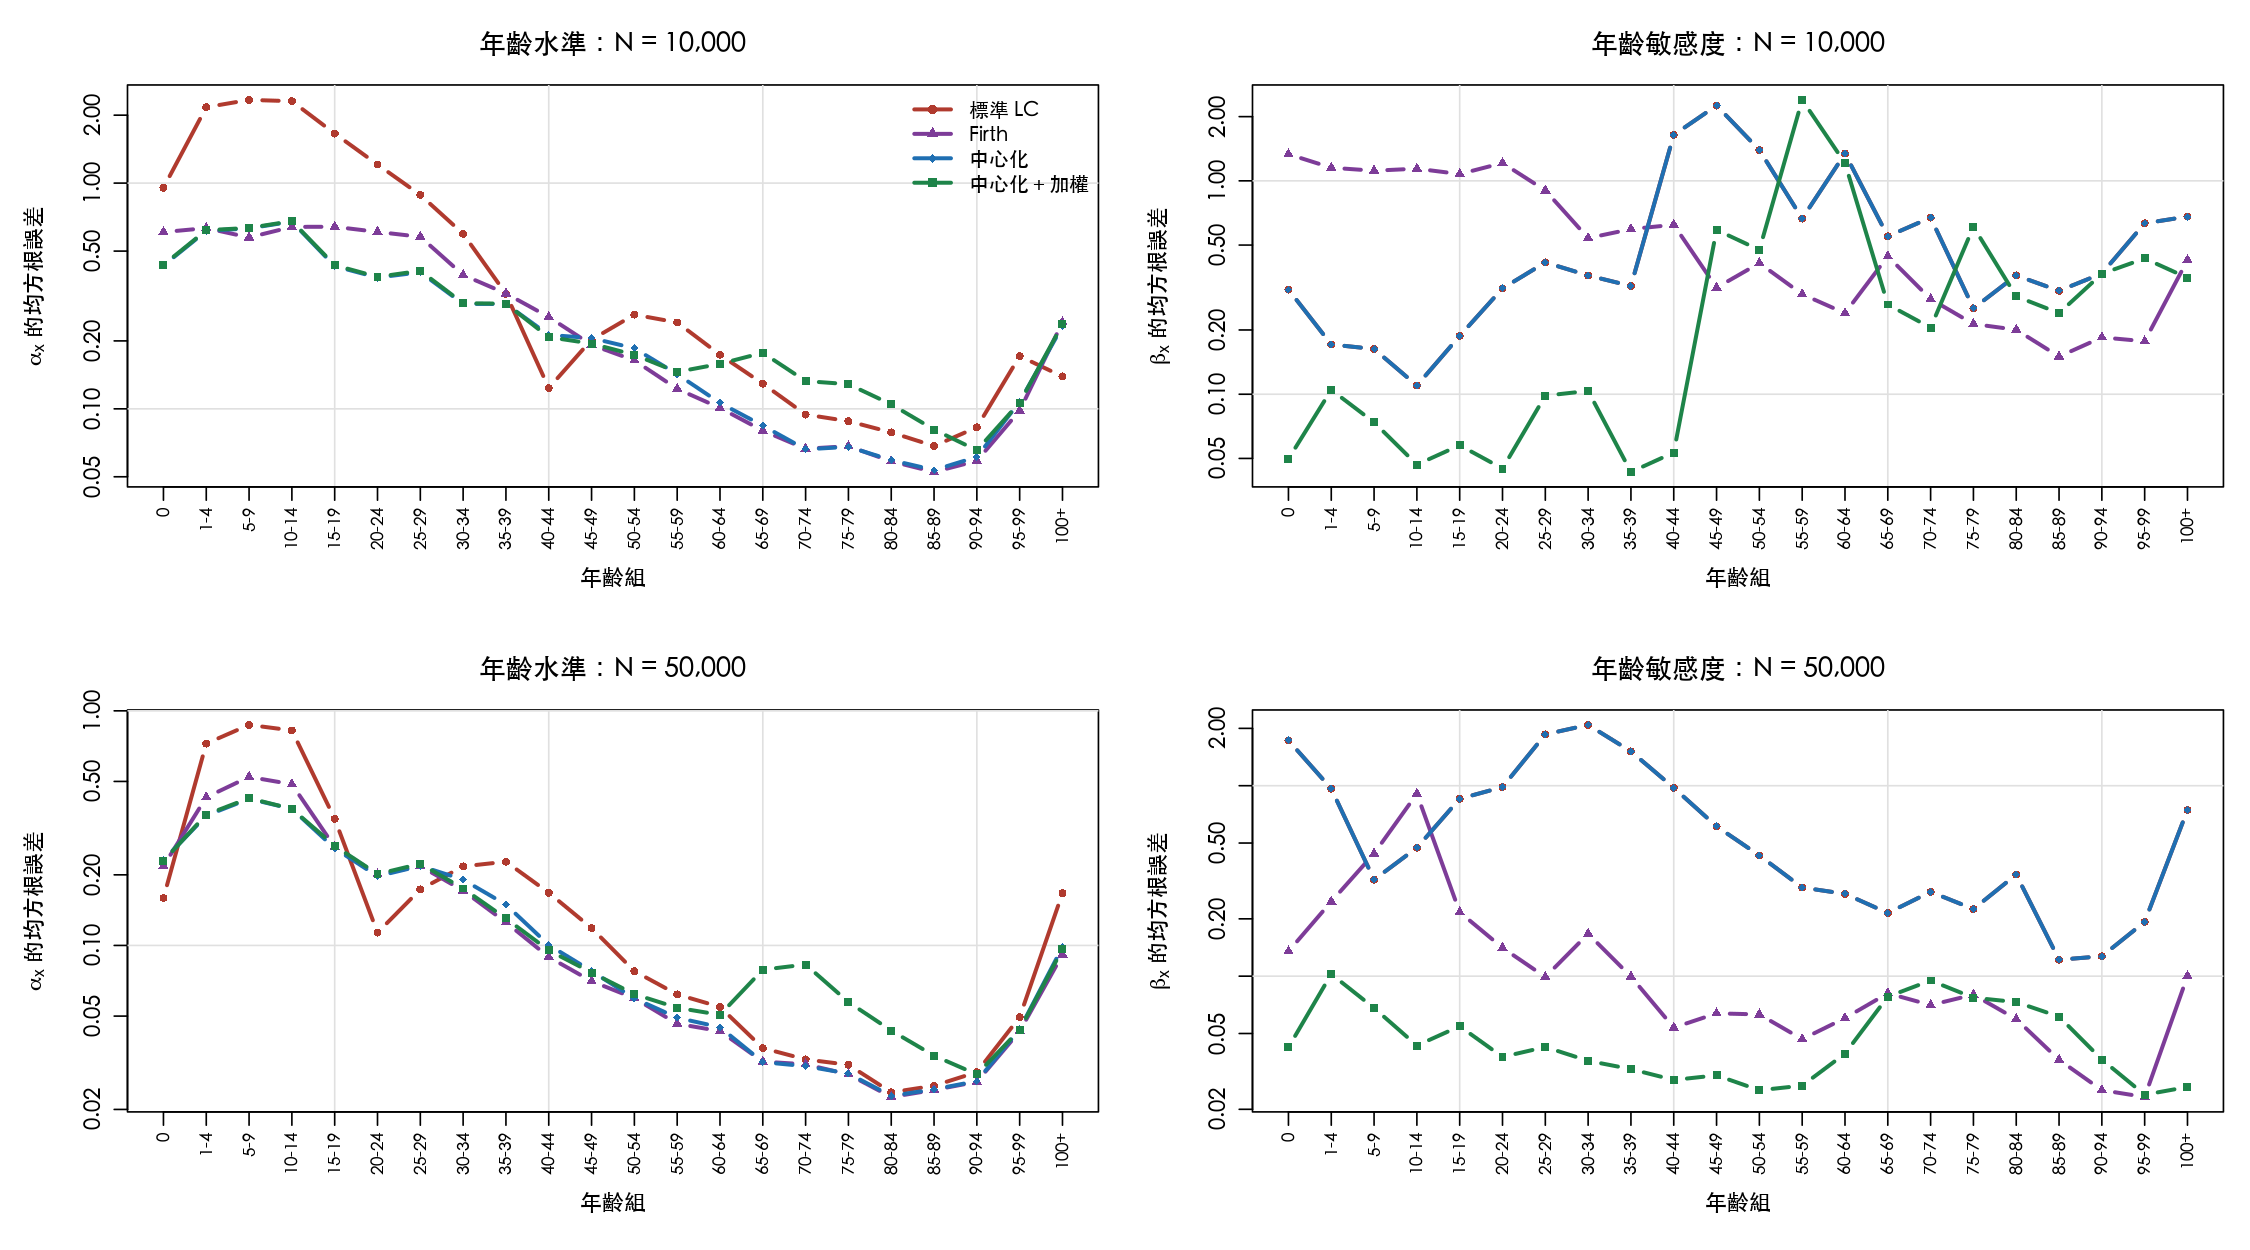
\includegraphics[width=0.82\textwidth]{figT9_age_profile.png}
\caption{校正的改善倍數隨年齡（人數五萬）}
\end{figure}

$\alpha$ 的改善集中在 $\mu$ 小的年齡（$0$ 至 $14$ 歲約 $1.9$ 倍），
$\beta$ 的改善遍及全齡（最高 $34$ 倍）；
而 $15$ 至 $34$ 歲因 $\mu\approx\mu^{\ast}$ 而幾乎沒有改善——
\textbf{該處本來就沒有偏誤可改}，與閉式的預測一致。

\subsection{已確定不可行的方向}

列出負面結果，以免重複投入。

\begin{itemize}
\item \textbf{不取對數並不解決小樣本問題。} 恆等轉換下估計方程恆為無偏
（$\Ex[D-\mu]=0$），故本文所研究的偏誤完全是轉換造成的；
但代價是解的存在性——人數一萬時 Poisson 最大概似的 $\alpha$ 最大偏誤為
$6.50$，且一百次重複中有 $93$ 次至少一個年齡落在邊界。
\textbf{偏誤由估計方程移到了解的存在性，而小樣本的困難主要在後者。}
\item \textbf{變異安定轉換可用而不宜為主。} Anscombe 尺度在人數一萬處
優於標準 Lee-Carter（$\alpha$ 最大 $2.33\to1.45$），但劣於 Firth（$0.18$）
與本文的分離式（$0.51$）。
\item \textbf{有界影響的截斷買不到東西。} 人數五萬時截斷是純粹的損失。
成因是病灶為\textbf{整列沒有資訊}而非少數離群值，
而截斷單一格無法替一個沒有資訊的列造出資訊。
\item \textbf{二階的插入式校正在數值上不穩定。} 插入式誤差可分解為
$b'(\mu)\mathrm{bias}(\hat\mu)+\tfrac12 b''(\mu)\mathrm{Var}(\hat\mu)$，
而兩項在幼年組幾乎互相抵銷（$1$--$4$ 歲：$-0.113$ 與 $+0.075$，實際 $+0.001$），
淨值落在三階。
\end{itemize}

\subsection{後續工作的優先序}

以下的排序刻意\textbf{把區間推論與真實次國家資料排除在可排程的工作之外}，
理由於本節末說明。

\begin{enumerate}[label=\arabic*.]
\item \textbf{$\kappa_t$ 與 $\beta_x$ 納入同一框架（最高優先）。}
$\hat\alpha_x$ 有恆等式而兩者沒有，因前者是列平均、後者是奇異向量與奇異值，
須以逐元而非子空間的擾動理論處理 \citep{abbe2020}。
校正後 $\beta$ 偏誤最大的年齡趨於穩定（$1$--$4$ 與 $70$--$74$），可為切入點；
而 $\kappa_t$ 在年金實務上是最關鍵的一條，第\ref{s:sol}節已顯示其
衰減與形狀誤差須分開處理。
\item \textbf{秩一是否足夠的檢定。} 本文全篇以秩一結構為前提而未檢定該前提，
而第\ref{s:strat}節末顯示偏離秩一時 $\alpha$ 的校正穩健、
$e_0$ 的好處則會消失，\textbf{故該檢定決定的是結論的適用範圍而非細節}。
可用的工具有兩類且成本皆低：非可加性的單自由度檢定，
以及以 Poisson 抽薄作交叉驗證來選因子個數。
\item \textbf{正規化改為單純形。} 依第\ref{ss:norm}節，
加上 $\beta_x\ge0$ 即可使可行集緊緻，
且因本文的 $\hat\beta_x$ 皆為正而不改動任何已報告的數值。
\textbf{成本最低而消掉一個結構性的病灶}，宜與第 1 項併行。
\item \textbf{混合設計。} $\alpha$ 與 $\beta$ 由對數尺度的分離式求得，
漂移改由計數尺度的擬分數估計——後者在人數五萬時把漂移偏誤清到約零
（$-0.004$ 對本文的 $+0.136$）。三個參數的作用域已證可分離，
故此種拼接在估計方程的層次上乾淨。
\item \textbf{偏誤定理與演算法定理的分離。} 本文的一階偏誤結果
不自動保證修正後的估計方程有唯一根、亦不保證任意起點下的迭代收斂；
兩者應在定理的陳述中分開，而第\ref{ss:norm}節的結果正是一個反例。
\item \textbf{插入式誤差的二階處理。} 依第\ref{ss:plugin}節，
兩項展開在幼年組幾乎互相抵銷而淨值落在三階，
故直接的二階校正不可行；可行的方向是降低 $\mathrm{Var}(\hat\mu)$
而不增加其偏誤。
\end{enumerate}

\textbf{兩項刻意排除，而理由不同。}

\textbf{其一，區間推論。} 這並非因其不重要——本文通篇為點估計而監理框架
要的是分布——而是因為\textbf{三條現成的路線目前各有一個否定的結果}：
Wald 區間因 $\partial b/\partial\log\mu\to-1$ 而不適用；
整列全零時任一精確信賴集合必有一個方向為無限長
（\citealp{lewis2024}，以先例引用）；
而偏誤不隨樣本量消失時，自助法所重現的是含偏誤的分布
\citep{cavaliere2024}，而本文的偏誤正是有限樣本的恆等式。
\textbf{在理論上找到一條可落地的路線之前，投入模擬是過早的}；
故本文的立場是先把這三項障礙寫清楚，待其一被解開再排程。

\textbf{其二，真實次國家資料。} 此項\textbf{不受本人進度控制}，
故應持續洽詢而不列入可排程的工作。在取得之前，
第\ref{s:prob}節的年齡結構分析與第\ref{ss:cross}節的跨國比較
是外部效度所能做到的上限——\textbf{而該節已明確寫出，
跨國所驗證的是閉式與門檻公式，不是實務表現}。

\subsection{適用的界限}

誠實的結論是\textbf{本方法把可用範圍往下推了，但沒有移除下限}。
人數一萬時所有方法都不足以支持單獨編表，最佳的均方根誤差仍有 $1.378$ 歲。
該下限有兩項一般性的理由：跨年齡合併所能換得的有效樣本量上限為
$(\sqrt T+\sqrt A)/\sqrt T$，在 $A=22$、$T=24$ 下為 $1.96$ 倍且會飽和，
而遷移學習的理論指出該上限會隨來源與目標的差距退化 \citep{reeve2021}；
又本文所查範圍內未見任何方法降低相變的可偵測門檻。

\textbf{關於秩一的依賴，已有量化的結果。}
以各國全國資料的第二個奇異成分為偏離的方向、強度掃 $0$ 至 $2$ 倍，
得兩項結論。其一，\textbf{$\alpha$ 的校正對偏離秩一穩健}：
改善倍數在 $4.2$ 至 $18.5$ 倍之間起伏而無趨勢。
此有先驗的理由——閉式所刻畫的是資料的列平均 $\overline{\log\max(D,c_0)}$，
其偏誤為 $\overline{b(\mu)}$，\textbf{與 $\log\mu$ 是否為秩一完全無關}；
秩一只透過插入的 $\hat\mu$ 進入，而 $b$ 在 $\mu$ 上平滑。
其二，\textbf{$e_0$ 的好處則隨偏離退化並會消失}：

\begin{table}[H]
\centering
\caption{受控偏離秩一下的表現（人數五萬）}
\small
\begin{tabular}{llrrrr}
\toprule
國家 & 第二成分佔比 & 標準 $\alpha$ 最大 & 分離式 & 標準 $e_0$ & 分離式 $e_0$\\
\midrule
臺灣 & 0.000 & 0.7896 & 0.0888 & $-1.440$ & $+0.489$\\
臺灣 & 0.043 & 0.7886 & 0.1282 & $-1.326$ & $+0.629$\\
臺灣 & 0.152 & 0.7876 & 0.0626 & $-1.354$ & $+0.715$\\
美國 & 0.000 & 0.6184 & 0.0723 & $+0.326$ & $-0.109$\\
美國 & 0.350 & 0.6159 & 0.0817 & $+0.903$ & $+0.609$\\
美國 & 0.683 & 0.6134 & 0.0380 & $\mathbf{+1.037}$ & $\mathbf{+1.427}$\\
\bottomrule
\end{tabular}
\label{t:rank2}
\end{table}

美國在第二成分佔 $35\%$ 時校正仍優於標準，佔 $68\%$ 時\textbf{反而較差}，
故交叉點落在三成五至六成八之間。
\textbf{亦即 $\alpha$ 層次的保證在模型誤設下存活，$e_0$ 層次的好處不然}，
這是把 $e_0$ 降為下游敏感度分析而非並列證據的理由。

另有兩項限制須明寫。其一，所提校正\textbf{依賴秩一雙線性結構}，
其程度如上段所量。
其二，時間參數的全距被壓縮，外推後將低估年金負債；
該項不在所提修正的涵蓋範圍內。

最後，\textbf{「Lee-Carter 實務上預測得好好的」這個質疑與本文並不衝突}：
預測表現良好與估計值不支持參數層次的詮釋可以同時成立
\citep{bratsberg2026}。本文所主張的始終是後者。

\subsection{三項貢獻的收束}

\begin{enumerate}[label=\arabic*.]
\item \textbf{把一個以模擬觀察到的現象化為恆等式。}
小人口 Lee-Carter 的 $\alpha$ 偏誤有閉式 $b(\mu;c_0)$，
為有限樣本的恆等式而非漸近近似，驗證的逐年齡相關係數為
$1.000$、$1.000$、$0.988$。
\item \textbf{由該閉式導出一個事前的可行性檢定。}
因偏誤只需曝露數與粗略死亡率即可算出，
該檢定不需模擬、不需真值、也不需參考母體，
並補上了信賴度標準所缺的偏誤側門檻。
\item \textbf{指出校正的正確施加位置。}
只校正 $\alpha$ 而以資訊加權處理秩一結構，兩項改善可以疊加，
而其成因是加權修正變異函數（一階）、中心化修正轉換的偏誤（二階），
兩者的作用域互不重疊且分離是精確的。
\end{enumerate}

\noindent（完整版第玖節）

\clearpage
\bibliographystyle{plainnat}
\bibliography{references}

\end{document}
